% TODO Remove when DONE
% Template Tutorial 
% https://www.overleaf.com/learn/latex/How_to_Write_a_Thesis_in_LaTeX_(Part_2):_Page_Layout


\documentclass[a4paper,12pt,twoside]{report}

\usepackage{algorithmic}
\usepackage{algorithm} 
\usepackage{array}
\usepackage{amsmath}
\usepackage{amsfonts}
\usepackage{amssymb}
\usepackage{amsthm}
\usepackage{caption}
\usepackage{comment} 
\usepackage{epsfig} 
\usepackage{fancyhdr}
\usepackage[T1]{fontenc}
\usepackage{geometry} 
\usepackage{graphicx}
\usepackage[colorlinks]{hyperref} 
\usepackage[latin1]{inputenc}
\usepackage{multicol}
\usepackage{multirow} 
\usepackage{rotating}
\usepackage{setspace}
\usepackage{subfigure}
\usepackage{url}
\usepackage{verbatim}
\usepackage{xcolor}
\usepackage{booktabs}
\usepackage{pythonhighlight}
\usepackage[nottoc]{tocbibind}
\usepackage[bottom]{footmisc}
% for the drawings
\usepackage{tikz}


\geometry{a4paper,top=3cm,left=2cm,right=2cm,bottom=3cm}

\pagestyle{fancy}
\fancyhf{}
\fancyhead[LO, RE]{\textsl{\leftmark}}
\fancyfoot[RO, LE]{Diploma 2019-2020}
\fancyfoot[LO, RE]{\thepage}

\renewcommand{\headrulewidth}{0.5pt}
\renewcommand{\footrulewidth}{0.5pt}
\renewcommand{\headrule}{\hbox to\headwidth{%
  \color{black}\leaders\hrule height \headrulewidth\hfill}}
\renewcommand{\footrule}{\hbox to\headwidth{%
  \color{black}\leaders\hrule height \footrulewidth\hfill}}

% Define special symbols
\newcommand{\CSharp}{{\settoheight{\dimen0}{C}C\kern-.05em \resizebox{!}{\dimen0}{\raisebox{\depth}{\textbf{\#}}}}}
\newcommand{\code}[1]{\texttt{#1}}

\providecommand{\keywords}[1]{\textbf{\textit{Keywords---}} \texttt{#1}}

\hypersetup{
	pdftitle={artTitle},
	pdfauthor={name},
	pdfkeywords={pdf, latex, tex, ps2pdf, dvipdfm, pdflatex},
	bookmarksnumbered,
	pdfstartview={FitH},
	urlcolor=cyan,
	colorlinks=true,
	linkcolor=black,
	citecolor=blue,
}

\setcounter{secnumdepth}{3}
\setcounter{tocdepth}{3}

\linespread{1}
\makeindex


\begin{document}

\begin{titlepage}
	\sloppy
	\begin{center}
		BABE\c S BOLYAI UNIVERSITY, CLUJ NAPOCA, ROM\^ ANIA

		FACULTY OF MATHEMATICS AND COMPUTER SCIENCE

		SPECIALIZATION COMPUTER SCIENCE IN GERMAN

		\vspace{0.5cm}
		
\includegraphics{figures/Logo_UBB.png}

		\vspace{5cm}
		\Huge \textbf{Cloud based malicious PDF Detection using Machine Learning}

		\vspace{1cm}
		\normalsize -- Diploma thesis --
	\end{center}

	\vspace{4cm}
	\begin{flushleft}
		\Large{\textbf{Supervisor}}\\
		Assoc. Prof. Christian S\u AC\u AREA
	\end{flushleft}

	% \vspace{5cm}
	\begin{flushright}
		\Large{\textbf{Author}}\\
		Viorel GURDI\c S
	\end{flushright}

	\vspace{2cm}
	\begin{center}
		2020
	\end{center}
\end{titlepage}

\pagenumbering{gobble}

\begin{abstract}
	PDF documents are one of the most popular file formats used for information exchange. People trust this format and open the files as soon as they come into their possession. Few know the risks to which they expose the integrity of their computers. For already many years PDF files became a frequently used attack vector for compromising the security of entire networks. This paper will introduce you into some of the currently known PDF attack techniques. Our work is aimed to research if the Machine Learning algorithms can successfully reinforce the classical antiviruses at analyzing malicious PDF documents. We provide an alternative security solution, which could take the responsibility of the hard task of malware analysis to an isolated, high-performant environment in the Cloud. Detected harmful PDF documents will be immediately removed from the computer and users should not worry about their data privacy nor computer performance. \\

	\keywords{Cybersecurity, Machine Learning, malicious PDF, Cloud Application}
\end{abstract}


\tableofcontents

\newpage

\listoftables
\listoffigures
% \listofalgorithms

\newpage

\setstretch{1.25}

\newpage

\pagenumbering{arabic}



\chapter{Introduction}
\label{chapter:introduction}

\section{What? Why? How?}
\label{section:what}

Motivate and abstractly describe the problem you are addressing and how you are addressing it. 
\begin{itemize}
	\item What is the (scientific) problem? 
	\item Why is it important? 
	\item What is your basic approach? 
\end{itemize}

A short discussion of how it fits into related work in the area is also desirable. Summarize the basic results and conclusions that you will present. 


\section{Paper structure and original contribution(s)}
\label{section:structure}

The research presented in this paper advances the theory, design, and implementation of several particular models. 

The main contribution of this report is to present an intelligent algorithm for solving the problem of $\ldots$.

The second contribution of this report consists of building an intuitive, easy-to-use and user
friendly software application. Our aim is to build an algorithm that will help $\ldots$.

The third contribution of this thesis consists of $\ldots$.


The present work contains $xyz$ bibliographical references and is structured in five chapters as follows.

The first chapter/section is a short introduction in $\ldots$.

The second chapter/section describes $\ldots$.

The chapter/section \ref{chapter:proposedApproach} details $\ldots$.



\chapter{Related work}
\label{chapter:relatedWork}
Beginning with the first reported occurences of malware, the security researchers have made a huge effort to prevent the harmful behavior. Over the years malware has evolved in different forms and of course the antivirus industry has developed more complex detection solutions. Since PDF documents became a good target for cybercriminals, more and more specialists pay attention to the analysis of dangerous PDFs. Integration of so many analysis tools in a single antivirus software has a negative impact on computers performance. For this reason, the cybersecurity field attaches importance to Cloud Computing. In the following sections we will analyze other academic and industrial approaches for transfering antimalware engines to the cloud and some docummented detection techniques of malicious PDFs.


\section{Cloud based malware detection}
\label{section:relatedWorkCloud}
In the field of Cloud solutions for malware detection, there is a sparse amount of shared academic works. As compensation, in the antivirus industry there is a fast growing interest for Cloud Computing, which has higher computational power and could therefore run more advanced and complex detection algorithms. \par
An important example is \textbf{VirusTotal} \cite{virustotal}, a popular Cloud application developed by Hispasec Sistemas, that aggregates more than 50 antivirus engines and makes them publicly available for scanning uploaded files. From the user perspective, this is an excellent application, that can extract metadata of the submitted file and can identify any dubious signal. The provided result represents a comparation between analysis verdicts of cybersecurity market leaders. Of course this is an advantage in terms of the scanning result precision and respectively a gain regarding spent computational time. On average it takes aprox. 55 seconds to upload and analyze a 400KB file. VirusTotal is also helping to maintain the global cybersecurity at a high level, by sharing all the submitted suspicious files with the security researchers. Thereby the antivirus engines will be permanently improved. \par
\textbf{Sandbox Analyzer} is another antimalware cloud solution developed by Bitdefender \cite{bdSandbox}. It's approach is a bit different, because it
ensures the security on a private network, where the Bitdefender product is installed, thus not being available for public access. It's operating principle is also specific, by preventing the execution of threats on an endpoint and automatically sending of harmful files to the Cloud. After extra analysis in the Cloud, the Sandbox Analyzer can take remediation action based on the verdict. In that way, malicious files get disinfected, quarantined or deleted. One of the benefits for this solution is in-depth analysis of malicious files in an isolated environment, rather than on user's machine. Thereby the risk for performance implication, as well as the risk of accidental run of malware on an endpoint machine are eliminated. At the core of the Sandbox Analyzer there are Machine Learning algorithms and dynamic behavior analysis techniques that are constantly improved to detect fresh threats.

% TODO maybe add this https://bradscholars.brad.ac.uk/bitstream/handle/10454/16043/Version%203.3%20-%20Thesis.pdf?sequence=1&isAllowed=y


\section{Detection of malicious PDF}
\label{section:relatedWorkML}
\textbf{PJScan}, presented in the paper of Laskov and Srndic \cite{pjscan}, is a Machine Learning approach that trains One-Class Support Vector Machine (\textit{OCSVM}) to classify PDF files. This approach is focused on static analysis of embedded Javascript code, as it is known for the ability of integrating malicious behavior in PDF documents. The authors used \textit{n-gram} analysis to extract lexical features, such as Javascript operators and other tokens. The obtained sequence of features served later as input for the machine learning algorithm. The trained model can correctly classify malicious samples containing Javascript code. However PJScan has a lower accuracy, because it is not able to detect obfuscated parts and there are also some samples containing other types of malicious payload, such as SWF\footnote{Adobe Flash file format used for multimedia}. \par
Another example of static analysis of PDF Structure is \textbf{PDF Tools} by Didier Stevens \cite{pdftools}. It represents a suite of tools for scanning, parsing and dumping PDF files. This approach focuses on identifying the fundamental elements of the format, such as Streams, Cross Reference Tables etc. The advantage of PDF Tools is their ability of name obfuscation handling and their simplicity. Because of their high speed performance, PDF Tools are largely used in cybersecurity research. \par
A completely new approach mentioned in the research paper of Fettaya et al. \cite{deepdf} describes an algorithm that uses a Convolutional Neural Network (\textit{CNN}) to detect malicious PDF files. The trained model, based on a single convolutional layer with a global max pool and a linear layer doesn't require any data preoprocessing. Instead of this, the model is trained using as input the binary representations of the files. It is worth noting that the described algorithm could be efficiently used for distinguishing various families of malware. The rate of correct detections achieves 94\%, the algorithm being also capable to classify aprox. 80\% of the malware into different categories.
\chapter{Scientific Problem}
\label{section:scientificProblem}

\section{Problem definition}
\label{section:problemDefinition}
The purpose of the research in this thesis consists in approaching some alternative methods to replace classic file scanning techniques. Particularly, our target is to demonstrate that Machine Learning algorithms can be used as an efficient mechanism for malicios PDF files detection. Additionally, we want to present a framework that can remotely analyze suspicious PDF files by applying earlier mentioned performant algorithms. This framework has several advantages: 
\begin{itemize}
    \item Takes on the complicated task of applying classification model for uploaded files and giving the analysis result to the users.
    \item It is designed to be deployed as a Cloud Application on a powerfull server that can handle multiple requests at the same time, lacking users care about having high specifications for their computers.
    \item Guarantees the privacy of the scanned documents. The algorithms doesn't require the documents content in order to decide whether they are malicios or benign. Also, after analysis process, none of the documents are stored on the Cloud.
    \item Keeps the detection algorithms up-to-date. It won't be the users responsability anymore to regularly update the software antivirus installed on their computers. 
    \item Provides a generic implementation for analyzing uploaded files. The support for a new file extension to be scanned, can be effortlessly added by adding a classifier Machine Learning model for the wanted file format.
\end{itemize}
Integrating both Machine Learning and Cloud Computing into Cybersecurity should provide a significant progress to this field. \par


In order to fully automate the process of detection malicious PDF files, our application provides a tool (currently has support only for Microsoft Windows) that independently uploads detected files to the Cloud Service, waits for analysis results and takes appropiate protective measures. In the following we will introduce some operating system concepts that helped us to achieve the expected behavior for our application.

\section{Background processes in Microsoft Windows}
\label{section:backgroundProc}
% https://www.2brightsparks.com/resources/articles/understanding-sessions-in-windows.html
In computing, a background process is a process\footnote{a container for a set of resources used when executing the instance of the program} that runs independently and doesn't require any user involvement. Usually it has the task of system monitoring and sending any types of notifications to the user. Each operating system has its own principle of implementation for background processes. We will have an in-depth look at background processes in Microsoft Windows, which are called \textbf{Windows Services}. According \cite{winInternals} these services are started by a central utility - \textit{Services Control Manager} at the boot-time\footnote{the period when a computer is starting} of the computer and they don't have any graphical interface. For security and safety reasons, specifically to prevent user applications from accessing Windows Services that could run with high privileges, Windows OS creates a new session for each logged in user, reserving \textit{Session 0} for non-interactive services. The mentioned features make Windows Services suitable for long-running functionality, whose operation doesn't interesect with other users work on the same computer. The support for creating a service is provided by \textbf{.NET Framework}, its features being possible to access by using one of Microsoft's high-level programming language \CSharp.

\section{File System monitoring}
\label{section:filesystem}
In the field of operating systems, a file system is aimed to store data in form of files in a long-term storage. Before being stored on physical devices, data that is created and saved by applications in User-Mode, goes through a chain of drivers from Kernel-Mode. This principle is adopted in many operating systems, inclusively in Microsoft Windows (see Figure \ref{filterDriver}). In order to track every change on the computer's file system, we need a monitoring mechanism. Throughout the development of Windows, serveral technologies have been implemented for integration by software engineers, including: File System Filter Drivers, Update Sequence Number Journal (\textit{USN Journal}), Event Tracing for Windows (\textit{ETW}), \textit{FileSystemWatcher} Class from .NET. In this section we are focusing on two of the most popular Windows file system monitoring mechanisms: Minifilter drivers managed by \textit{Filter Manager} and \textit{FileSystemWatcher}. \par
\textbf{Windows Filter Manager} is a Kernel-Mode driver that intercepts every file system I/O operation and can extend the functionality of the requested operation through each minifilter driver that is registered to it (see Figure \ref{filterDriver}). The order of attachement of each minifilter is identified by an altitude\footnote{unique identifier assigned by Microsoft that determines when a minifilter is loaded}, thus avoiding interleaving the functionality of callback routines of each minifilter. Windows Driver Kit (\textit{WDK}) provides the necessary SDK\footnote{collection of software development tools} for developing minifilter drivers, which are most suitable for Backup agents, Encrpytion managers and Antivirus filters. For more details consult \cite{msdn}. \par

\begin{figure}[H]
	\centerline{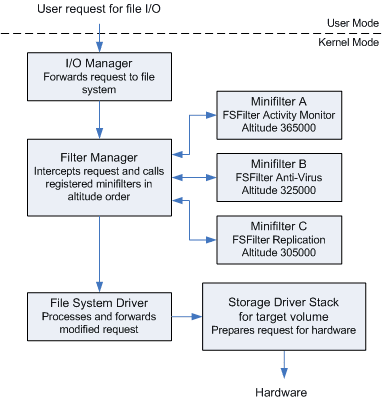
\includegraphics[scale=0.6]{figures/filterDriver.png}}  
	\caption{Simplified I/O stack from Windows \cite{msdn}}
	\label{filterDriver}
\end{figure}

Compared to the previous described technology, which is complex for development and mantaining, \textbf{FileSystemWatcher} is a class from .NET that makes file system monitoring straightforward to implement. According to \cite{dotNetFramework}, this class represents a wrapper over Win32 SDK \textit{ReadDirectoryChangesW} function, which is also used by Windows Explorer to monitor folder changes. By being provided by .NET, it is clear, that FileSystemWatcher can be used in User-Mode for development (see Figure \ref{netFramework}). 

\begin{figure}[H]
	\centerline{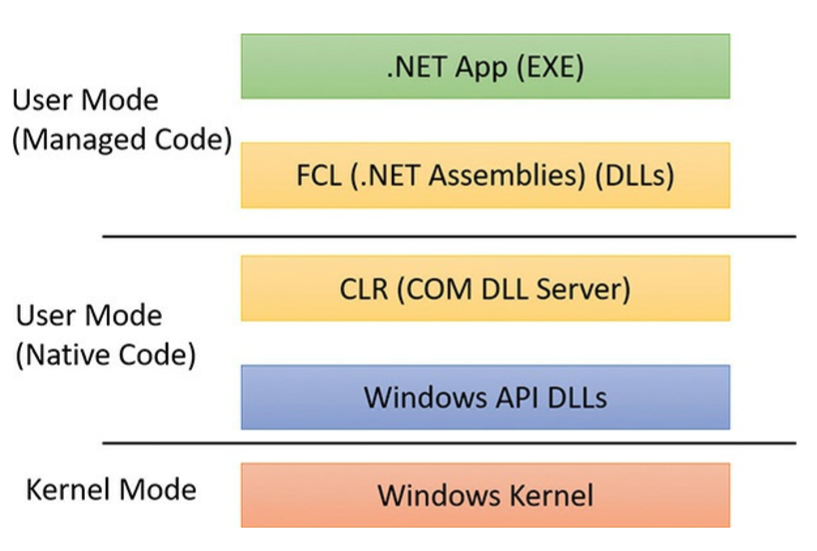
\includegraphics[scale=0.5]{figures/NetFramework.png}}  
	\caption{Relationship between .NET and Windows OS \cite{winInternals}}
	\label{netFramework}
\end{figure}

To configure a working instance of this class, we need to specify a couple of properties, such as \textit{Path} (for indicating the folder to monitor), \textit{NotifyFilters} (for specifieng what kind of file changes to monitor) and \textit{EnableRaisingEvents} (to start/stop monitoring process). Also we need to attach the corresponding events that we want to receive (see Table \ref{supportedEvents}).

\begin{table}[H]
	\caption{Events supported by FileSystemWatcher}
	\label{supportedEvents}
		\centering
            \begin{tabular}{l | l}
                
				\textbf{Event} & \textbf{Occuring time} \\
				\hline
 				Created & When a new file is created or is moved into monitored folder \\
 				Changed & When a file has its content or file attributes modified \\
 				Deleted & When a file is removed or is moved out of monitored folder \\
                Renamed & When the name of the file get changed\\
                 
			\end{tabular}
\end{table}

Earlier we mentioned that minifilter drivers live in Kernel-Mode, while FileSystemWatcher provided by .NET lives in User-Mode. One more argument in favor of FileSystemWatcher, besides the high level object-oriented programming language \CSharp that we have at our disposal over unmanaged\footnote{code executed directly by OS; does not provide any security to the application} C language, is that it's safer to run applications in User-Mode. Each application runs in isolation in User-Mode and in case of a crash, it won't affect other applications or even worse the OS itself, what can happen with a Kernel-Mode driver.

\section{Analyzing PDF File Structure}
\label{section:pdfStructure}

% $\ldots$ (see Figure \ref{pdfSkeleton})

% \begin{figure}[H]
% 	\centerline{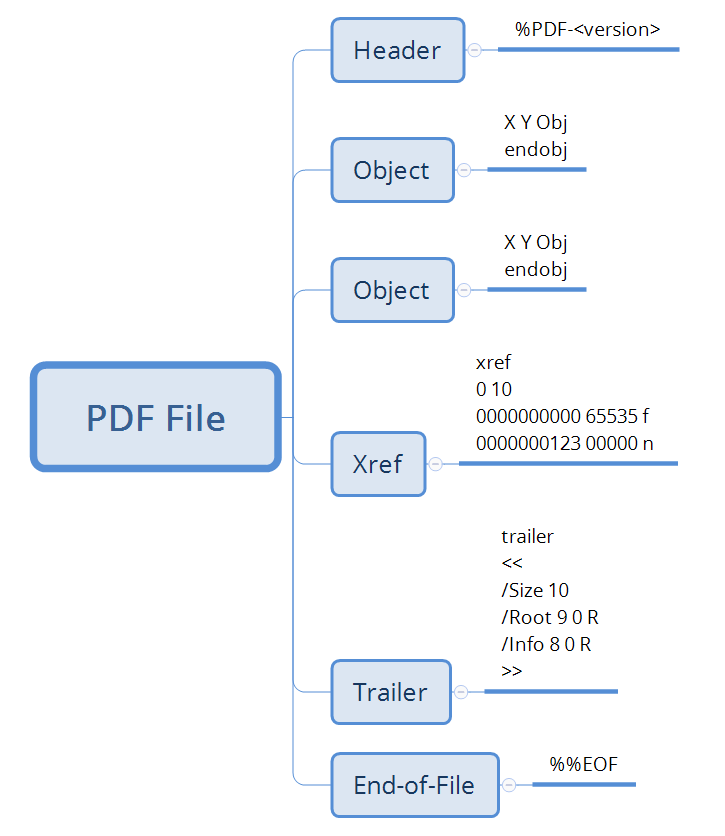
\includegraphics[scale=0.5]{figures/PDFSkeleton.png}}  
% 	\caption{Structure of PDF Format \cite{winInternals}}
% 	\label{pdfSkeleton}
% \end{figure}


\section{Malware in PDF}
\label{section:malwareInPDF}
% Since PDF documents became a well known solution for information sharing, they also became a good target for cybercriminals.

\section{Machine Learning for Malware Detection}
\label{section:mlForMalware}

\section{Benefits of Cloud Computing}
\label{section:cloudComputing}
% Using a cloud-based anti-virus makes it much easier to manage, especially as there's no need to constantly update software on multiple devices. However, it is worth bearing in mind that installing anti-virus to combat malware can only be one part of an overall IT security policy.
% https://www.redhat.com/en/topics/cloud-native-apps/what-are-cloud-applications
% Simply put, a cloud application is software that users access primarily through the internet, meaning at least some of it is managed by a server, not the user’s local machine. This basic definition doesn’t fully describe how cloud applications have reshaped markets and business models, though. If designed well, cloud applications can offer a user experience like a program installed entirely on a local machine, but with reduced resource needs, more convenient updating, and the ability to access functionality across different devices.
% Nowadays with cloud use being common, it's more efficient to install anti-virus software on your network.
% benfetis - low performant devices + mobile
% http://lxiao.xmu.edu.cn/Papers/Mobile%20Offloading%20for%20Cloud-based%20Malware%20Detections%20with%20Learning.pdf
%Advantages:
% Fast computation to run more advanced and complex detection algorithms
% More accurate detection with a large-size signature database
% Address zero-day vulnerabilitie
% Cloud-based malware detection vs. local detection
%  Transmission delay, computation speed, detection accuracy, storage cost
%  User competition vs. cooperation in the malware detection
%  Compete for the limited network bandwidth
%  Contribute the malware signature database to improve the malware
%  detection accuracy at the cloud
%Cloud computation resource=1Gbps
% Trace generation speed=1Mbps
% Transmission cost factor=0.2
% Accuracy coefficient=0.5 
\chapter{Proposed approach}
\label{chapter:proposedApproach}

For solving the problem of detecting malicious PDF documents, we came with a Machine Learning based approach. We took into account the importance of keeping the documents content confidentiality, as well as the need for ensuring the speed of analysis process. This solution will be next integrated into a Cloud framework responsible for remote documents scanning.

\section{Dataset}
\label{section:dataset}
The first step in building the optimal \textit{ML} model was to create a dataset which would train the classifier. Our target was to collect malicious and benign PDF samples used in real life scenarios. Circa 70\% of the clean and malicious documents were downloaded from the online malware repository \textit{Contagio} \cite{contagio}, which provides samples collected from various open sources. Nevertheless, for more recent malicious PDFs we used VirusTotal \cite{virustotal}, Hybrid Analysis \cite{hybridanalysis} and VirSCAN \cite{virscan}, that allow searching files by their hash (\textit{MD5}, \textit{SHA1}, \textit{SHA256}). Some of them provide access to the entire file collection so that we can order them by upload date and search for the most recent uploaded harmful files. Many clean samples were collected from public sources using Google Search Operators, i.e., \code{filetype:pdf}, for restricting search results of PDF files. Additionally, we completed the dataset with more than 100 clean interactive PDF files, that contain embedded 3D Widgets, incorporated JavaScript games etc. These clean samples should train the ML model, so as to correctly classify files even in corner cases. 

\begin{table}[H]
	\caption{Dataset of PDF samples}
	\label{table:pdfSamples}
        \centering
            \begin{tabular}{p{2.5cm} p{9.5cm}}
                \toprule
                
				\textbf{Category} & \textbf{Source} \\
				\hline 
                \texttt{benign} & Contagio, Google Queries, Tetra4D, PdfScripting \\
                \hline
				\texttt{malicious} & Contagio, VirusTotal, Hybrid Analysis, VirSCAN \\
                
                \bottomrule
			\end{tabular}
\end{table}

\section{Proof of Concept}
\label{section:poc}

In the following subsections we will touch upon algorithms and techniques we have used to achieve the purpose of this thesis, namely detecting malicious PDF documents using a Machine Learning based solution. Figure \ref{mlsteps} represents the entire process which was followed while developing the \textit{ML} model. Each process phase will be fathomed in the following.

\begin{figure}[H]
	\centerline{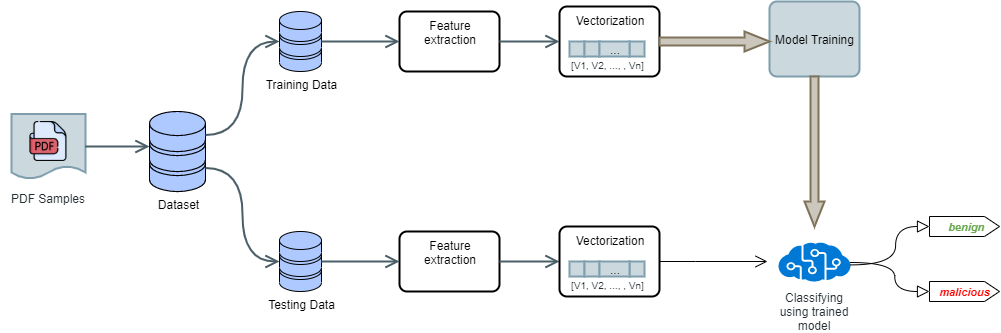
\includegraphics[scale=0.5]{figures/ml.png}}  
	\caption{Machine Learning model creation}
	\label{mlsteps}
\end{figure}

\subsection{Feature Selection}
\label{subsection:featureSelection}
As we already know, Machine Learning is based on mathematical concepts, hence the algorithms consist of performing mathematical operations to identify patterns in data. In order to use our dataset as input for ML algorithms, first of all we need to bring the data in an appropiate form. Therefor the most relevant data from a PDF document should be extracted and transformed into a vectorized form. As already seen in Table \ref{table:pdfentries}, there are several standard PDF entries which can be used for malicious intentions. For featurizing PDF documents we have used \textit{PDFiD} from \textit{PDF Tools} suite \cite{pdftools}, which is a Python script that selects 22 features from a PDF file, including keywords commonly found in malicious documents, name obfuscations etc. The output of the script is a list of PDF entries and their occurences (see Figure \ref{pdfidoutput}). Before turning this featurized form of the PDF file into input for ML algorithms, the data should be normalized to [0, 1] range. This is an important step in order to avoid ML issues when features are on drastically different scales (see \cite{mlCookbook}). The vectorized form of the PDF document is built by applying the \textit{Min-Max Normalization} (\ref{eq:1}) strategy on the array of features extracted by \textit{PDFiD}.

% In case of lack of content: Tell about multithreaded data mining

\begin{equation}
	\label{eq:1}
	z = \frac{x - min(x)}{max(x) - min(x)}
\end{equation}

\begin{figure}[H]
	\centerline{\includegraphics[scale=0.6]{figures/pdfidoutput.png}}  
	\caption{Example of results of \textit{PDFiD} applied on a benign PDF file (left) and on a malicious one (right)}
	\label{pdfidoutput}
\end{figure}

\subsection{Classification Technique}
As we have successfully created the dataset by vectorizing each PDF from our collection and setting a label for each one (everything saved as a CSV file), the next steps would be feeding the dataset to a ML classifier and training a model. According to our application's requirements, a PDF file should pass through a binary classification, so the analyzed files can be only \texttt{malicious} or \texttt{benign}, respectively a supervised strategy was chosen. The model, that is the goal of creation when applying Machine Learning, is able to perform tasks that it has not been explicitly implemented to execute. First of all we splitted the dataset into training data and 30 \% were allocated for testing data. The training data is used to fit the model, so that the resulting trained model could be used to predict the correct verdict on previously unseen metadata. \par 
Above all existing classification algorithm, \textbf{Random Forests} was selected because of its effective classification capability and the ease of use. Under the hood, this algorithm gives the classification result based on ensembling the results from multiple decision trees. First a random subset from training data is selected. At each split point $m$ features from $n$ available are randomly selected ($m \leqslant n$) and the optimal split point from $m$ features is picked ($m = \sqrt{n}$ is recommended). This step is repeated until an individual tree is trained and each result represents the vote of a decision tree. These votes are combined to give an unified final classification result of the Random Forest technique.
Even the training process is computationally expensive, once the classification model is constructed, categorizing is quickly executed. In order to make our API, that integrates this model, more efficient, we used the Python module - \texttt{pickle} to dump the virtual model into a file saved to disk. The process of refitting the model before using it to predict is much more time consuming than just loading the already fitted model form the disk.


\subsection{Experiment}
Before putting the chosen classification algorithm into work we definetely had to take several aspects into consideration. The most important of them is the environment where the model is trained. When working with malicious samples it is crucial to ensure that the personal computer integrity will not be affected. The instructions defined in Lenny Zeltser's articles \cite{zeltser} helped us to set up an isolated laboratory environment for our \textit{experiment}. First of all we used VMware to create a virtual machine (VM), where we installed a Linux distribution. In this way no physical machine could be damaged and the lightweight OS keeps the performance unimpacted. For further performance evaluations the allocated hardware specifications for the VM should be taken into consideration: \textit{RAM = 3GB}, \textit{CPU = 4 processor cores}. The communication with the development computer is through a shared folder, where the collection of PDFs, as well as the source code for training model were dropped. After configuring all the required libraries, the network adapter of the VM was completely removed, so that it could not establish any conexion to external sources in case of any malicious behavior. Also a snapshot of the set up environment was taken. This is another huge advantage of a virtual machine: in case of accidental opening of a malicious file, we could easily revert to a safe snapshot. \par 
After the classification model was successfully created, we decided to simulate a cyberattack using a malicious PDF file, in order to test the model prediction in a pseudo-real life scenario. Metasploit\footnote{a penetration testing framework} was used for injecting a malicious payload into an innocent looking file. After uploading the file to our analyzer, the classification result was as expected - \texttt{malicious}.


\subsection{Performance Evaluation}
As performance estimators for evaluating the strengths of the obtained classification model we have selected the following metrics, where \textit{TP} stands for True Positives, \textit{FP} - False Positives, \textit{FN} - False Negatives and \textit{TN} - True Negatives: 

\begin{equation}
	Accuracy = \frac{TP + TN}{TP + TN + FP + FN}
\end{equation}

\begin{equation}
	Recall = \frac{TP}{TP + FN}
\end{equation}

\begin{equation}
	F1-Score = \frac{2 \cdot Precision \cdot Recall}{Precision + Recall}
\end{equation}

Additionally we generate a confusion matrix to observe the presence of FP and FN.

% Add confusion matrix


% Classifier Performance Comparison + maybe add SVM (file:///C:/Users/viorel/Desktop/Bachelor/Resources/Malicious_PDF_Detection_ACSAC_12.pdf)


\section{Used technologies}
\label{section:technologies}
\subsection{Microsoft .NET Framework}
As previously mentioned in sections \ref{section:backgroundProc} and \ref{section:filesystem}, our application is going to have a help tool for Windows based computers that will automatically detect new downloaded PDF documents, upload them to our Cloud Analyzer and take action (keep/delete) on that files corresponding to their category (benign/malicious). This tool will take the form of a Windows Service which will start running at the boot-time of the computer in the Session 0 (see section \ref{section:backgroundProc}) and will communicate with an application responsible for notifying users through Windows notifications (see Figure \ref{winserviceDesign}). 

\begin{figure}[H]
	\centerline{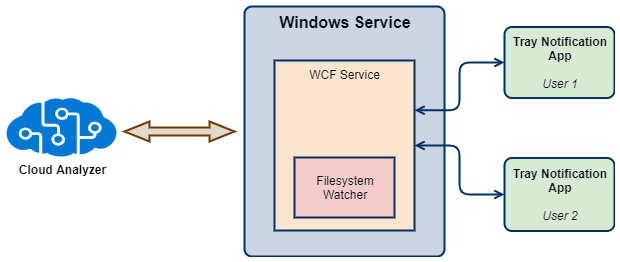
\includegraphics[scale=0.6]{figures/winService.png}}  
	\caption{Architecture's outline of the help tool for Windows}
	\label{winserviceDesign}
\end{figure}

Microsoft \textbf{.NET Framework} provides all the necessary Classes for creating the described tool. This framework represents a solution for standardization of application development on Windows operating system. Prior to the introduction of .NET Framework, the developers mostly used COMs\footnote{Component Objcet Model (COM) is a model of reusable software introduced by Microsoft in 1993} as a solution for code reuse. However, COM requires developers to write boilerplate code in order to turn their business logic into a reusable component, including memory clean up, reference counting etc, whence result a lot of errors. .NET Framework allow developers to focus on writing the business logic, while it is dealing with the memory management and is providing consistent exception-handling mechanisms. For example, in our application we implemented several .NET interfaces to achieve the expected behavior without having to manage a lot of low-level details. To create a Windows Service, we derived our class from \code{System.ServiceProcess.ServiceBase} and we had to override it's \code{OnStart}, \code{OnStop} methods. Because a service runs in Session 0, it means that it does not have support for user interface. Yet the application is intended to push Windows notifications and to ensure this functionality we had to treat our tool as a client-server application. The Windows service establishes an interprocess communication with the client \textit{Tray Notification App} when a user logs in. For this mechanism the WCF\footnote{Windows Communication Foundation (WCF) is a set an API in the .NET Framework for building connected, service-oriented applications} framework is integrated, which allows sending data as asynchronous messages from one endpoint to another. WCF was chosen as communication layer because it provides the \textit{duplex} message exchanging pattern, where two processes establish a secure TCP connection and can send data in both directions. To make this working, it is necessary to just define used entities for communication as \textit{Data Contracts}, that will later serialize the metadata by the WCF serialization engine. Another important component that lies at the core of the WCF service is the monitor class that inherits from .NET \code{System.IO.FileSystemWatcher}. It's behavior was described in section \ref{section:filesystem} and basically we use it to monitor user's specified folders and to send events to the users via the WCF communication. At the top level, in order to catch sent events from the Windows Service, a hidden WPF\footnote{Windows Presentation Foundation (WPF) is a UI framework for desktop applications from .NET Framework} application starts communication with the service at the user's login. When a PDF document is downloaded into monitored folder the Windows Service throws an event that is displayed to the user in form of a Windows System Tray Notification.


\subsection{Scikit-learn Machine Learning Library}
It would be extremely inefficient to always reimplement each Machine Learning algorithm that is required for solving a specific problem. \textbf{Scikit-learn} is one of the well known and largely used ML libraries, that came across as a solution for code reusability and performance optimization. This open-source library was created above the already prepared "ecosystem" for Data Science - \textit{Python}. Even Python is just a programming language, there are a plenty of created libraries using Python, that are used on a daily basis by scientists. In terms of efficiency there are no doubts, that Scikit-learn would give way to other ML libraries. And all this beacause of it's underlying technologies. At the core it integrates:

\begin{itemize}
	\item \textit{Cython} - a compiled language that can bind compiled libraries, reaching high performance of the CPU;
	\item \textit{Numpy} - optimized Python module for working with large multidimensional arrays;
	\item \textit{Scipy} - a large collection of efficient algorithms for linear algebra, interpolation etc.
\end{itemize}

Till now, the Scikit-learn developers have supplied the library with various supervised and unsupervised algorithms, such as: regression, clustering, classification algorithms, as well as: Random forest, Support Vector Machine etc. It is a perfect solution for both academic and commercial projects, because of the simple API that it provides, thus the generic implementation of the ML algorithms can be adapted to personal purposes. Also, Scikit-learn integrates well with other Python libraries, that consistently simplify the data analyisis process. Some of these libraries are: 

\begin{itemize}
	\item \textit{Pandas} - offers optimized data structures (\textit{DataFrames}) for manipulation of large datasets. We could simpy apply \textit{Min-Max Normalization} (see \ref{subsection:featureSelection}) on entire loaded dataset from a raw CSV file.
	\item \textit{Matplotlib} - used for data visualization and plotting. Learning Curves of the classifier can be better analyzed from a visual representation.
\end{itemize}


\subsection{Python Flask}
As soon as the heart of our application came to life - the ML model for detecting malicious PDFs we needed a way to make it publicly accessible. \textbf{Flask} is a microframework for web applications that helped us to make it possible. Comparing to other web frameworks, Flask is focused more on simplicity and extensibility, making the development much more oriented on solving own business case. This lightweight framework has no in-built database abstraction layer or object-relational mapping and neither any form validation or authentication, instead it supports third-party libraries that provide all enumerated functionalities and even more. Flask core includes basic functionality required by all web applications and gives an abstraction for creating request-response mechanism based on \textit{Werkzeug} library, which provides a collection of utilities for WSGI\footnote{Web Server Gateway Interface (WSGI) is a specification that describes the communication pattern between a web server and web applications} applications. Other implementation details can be easily integrated based on personal preferences. For example we used a NoSQL database in our application, having the possibility to choose from a large variaty of available mechanisms for data storage. \par
The created web service respects the requirements of a RESTful architectural design, Flask framework providing a simple mechanism for specifying routing and HTTP methods. For demonstration purposes we have listed below a minimalistic example of a REST HTTP Method (processes a file sent over a POST request and returns a JSON result) showing the Flask simplicity. One of the major advantages of this framework is the compatibility supported by nowadays giants of Cloud Computing. Our created web framework that exposes methods for uploading and PDF files and analyzing them, as well as visualizing history of scanned files, can be later deployed to Cloud services such as: Google Cloud Platform, IBM Bluemix, Microsoft Azure etc. \\

\begin{python}
from flask import Flask, jsonify, request
app = Flask(__name__)

@app.route('/api/file-upload', methods=['POST'])
def upload_file():
	file = request.files['file']
	file_status = file_controller.upload(file)
	response = jsonify({'message': file_status})
	response.status_code = 200
	return response

if __name__ == "__main__":
    app.run()
\end{python}


\subsection{ReactJS Framework}
In order to use the web service in a user friendly way, a modern graphical user interface (\textit{GUI}) is needed. The contemporary approach for developing a web GUI is to use a frontend JavaScript Framework. The range of choice is extremely large, e.g. \textit{Angular}, \textit{Vue.js}, \textit{Ember.js} etc., but finally we decided for \textbf{ReactJS}. Being deveveloped and mantained by Facebook, ReactJS has a fast growing community and is one of the trending JavaScript Frameworks for 2020. The need of using a framework for web GUI arises because of necessity for time-efficient development experience, standardized methods of programming, faster performance and robust memory management. As other frameworks, ReactJS is aimed to render data to the \textit{DOM}\footnote{Document Object Model (DOM) is the representation of a web page that can be manipulated using JavaScript} and to eliminate the subsequent page refreshes in a complex web application that constantly updates its data. This mechanism is provided by the concept of \textit{Virtual DOM} used in React, which involves constructing the representation of a web page in a virtual memory, where it uses the \textit{Reconciliation Algorithm}\footnote{is a diffing algorithm that compares the types of root elements and decides which element should be rerendered} to perform only the necessary updates before rendering the page into the browser. \par
The extensibility of React code is assured by \textit{Components}, that are rendered to specific elements in the DOM. These can be declared in two ways: functional and class-based, the main difference being in the "state" which can be hold only by a class-based component. The performance is influenced positively by the lifecycle methods in React Components. There are multiple lifecycle methods for controlling the state of a web page, but two of them that should be definetely took into consideration are \texttt{componentDidMount}, that is called once the data is fully loadded from a remote source, and \texttt{render} which is called every time the component's state gets updated. \par
Usually React requires the use of additional libraries for common functionalities like routing, state management and layout styling of the UI. For these purposes we used:

\begin{itemize}
	\item \textit{React Router} - is a routing library that keeps the user interface in sync with the corresponding URL. It manages the redirection, lazy code loading and dynamic route matching.
	\item \textit{Redux} - is a state management tool, that keeps tracking of each component's state and store them into a global place, so that data becomes more accessible from any component.
	\item \textit{Semantic-UI-React} - is a collection of UI standards defined as a singular style. Instead of recreating the layout of commonly used web elements (Buttons, Grids, Modals, Input Fields etc.), it is more efficient to use a library with all of those elements already created.
\end{itemize}



\chapter{Application}
\label{chapter:application}


\section{Design}
\label{section:design}

\section{Windows Service}
\label{section:winService}

% Before putting to disposition of the user this tool, we had to create an installer (++ winService)

\section{Cloud API}
\label{section:cloudApi}

\section{Dashboard Interface}
\label{section:dashboard}
\chapter{Conclusion and future work}
\label{chapter:conclusion}

The main objectives behind proposed approach for creating a Cloud application, which could scan PDF documents and return a verdict was successfully fulfilled. This paper demonstrates the capabilities of Machine Learning algorithms applied on cybersecurity tasks, which in some cases can provide even better results than a classic antivirus application. In addition to the Machine Learning framework responsible for PDF scanning, we also provide an automated solution for file uploading, which can take an according action to the scanned file based on it's result, in order to assure the safety of user's computer. The symbiosis of these two creates a complex system that distributes the performance-expensive task of malware analysis from an endpoint machine to a remote server. This way the user should not worry that his computer will be compromised by any PDF document, which these days is one of the most exchanged file formats. \par 
The next steps in extending our created product, will be making the framework publicly available, by deploying it on a Cloud service. Currently the automatic file uploader is supported only on Windows OS and the users have the alternative to manually submit the URL of a PDF file in order to scan it. In the future we plan to develop a similar background application for automating file upload for Android OS and possibly other operating systems. The Cloud application is also included in our upgrades plan. It's architecture already permits integrating of other Machine Learning models for classification of new file formats. The purpose of the upcoming research will be Microsoft Office Document formats (DOC, XLS, PPT), as well as PE (Portable Executable) and DLL (Dynamic-link library) files. \par
We think that now is the era for transfering all of the performance draining applications to the Cloud.


\bibliographystyle{plain}
\bibliography{BibAll}

\end{document}